\documentclass{article}

\usepackage{graphicx}
\usepackage{tikz}
\usepackage{tikzsymbols}
\usetikzlibrary{calc,patterns,shapes.geometric}
\pagestyle{empty}
\usepackage[margin=0pt]{geometry}
\geometry{papersize={14in,12in}}

\def\centerarc[#1](#2)(#3:#4:#5){\draw[#1] ($(#2)+({#5*cos(#3)},{#5*sin(#3)})$) arc (#3:#4:#5);}

\begin{document}
	\begin{figure}
		\centering
		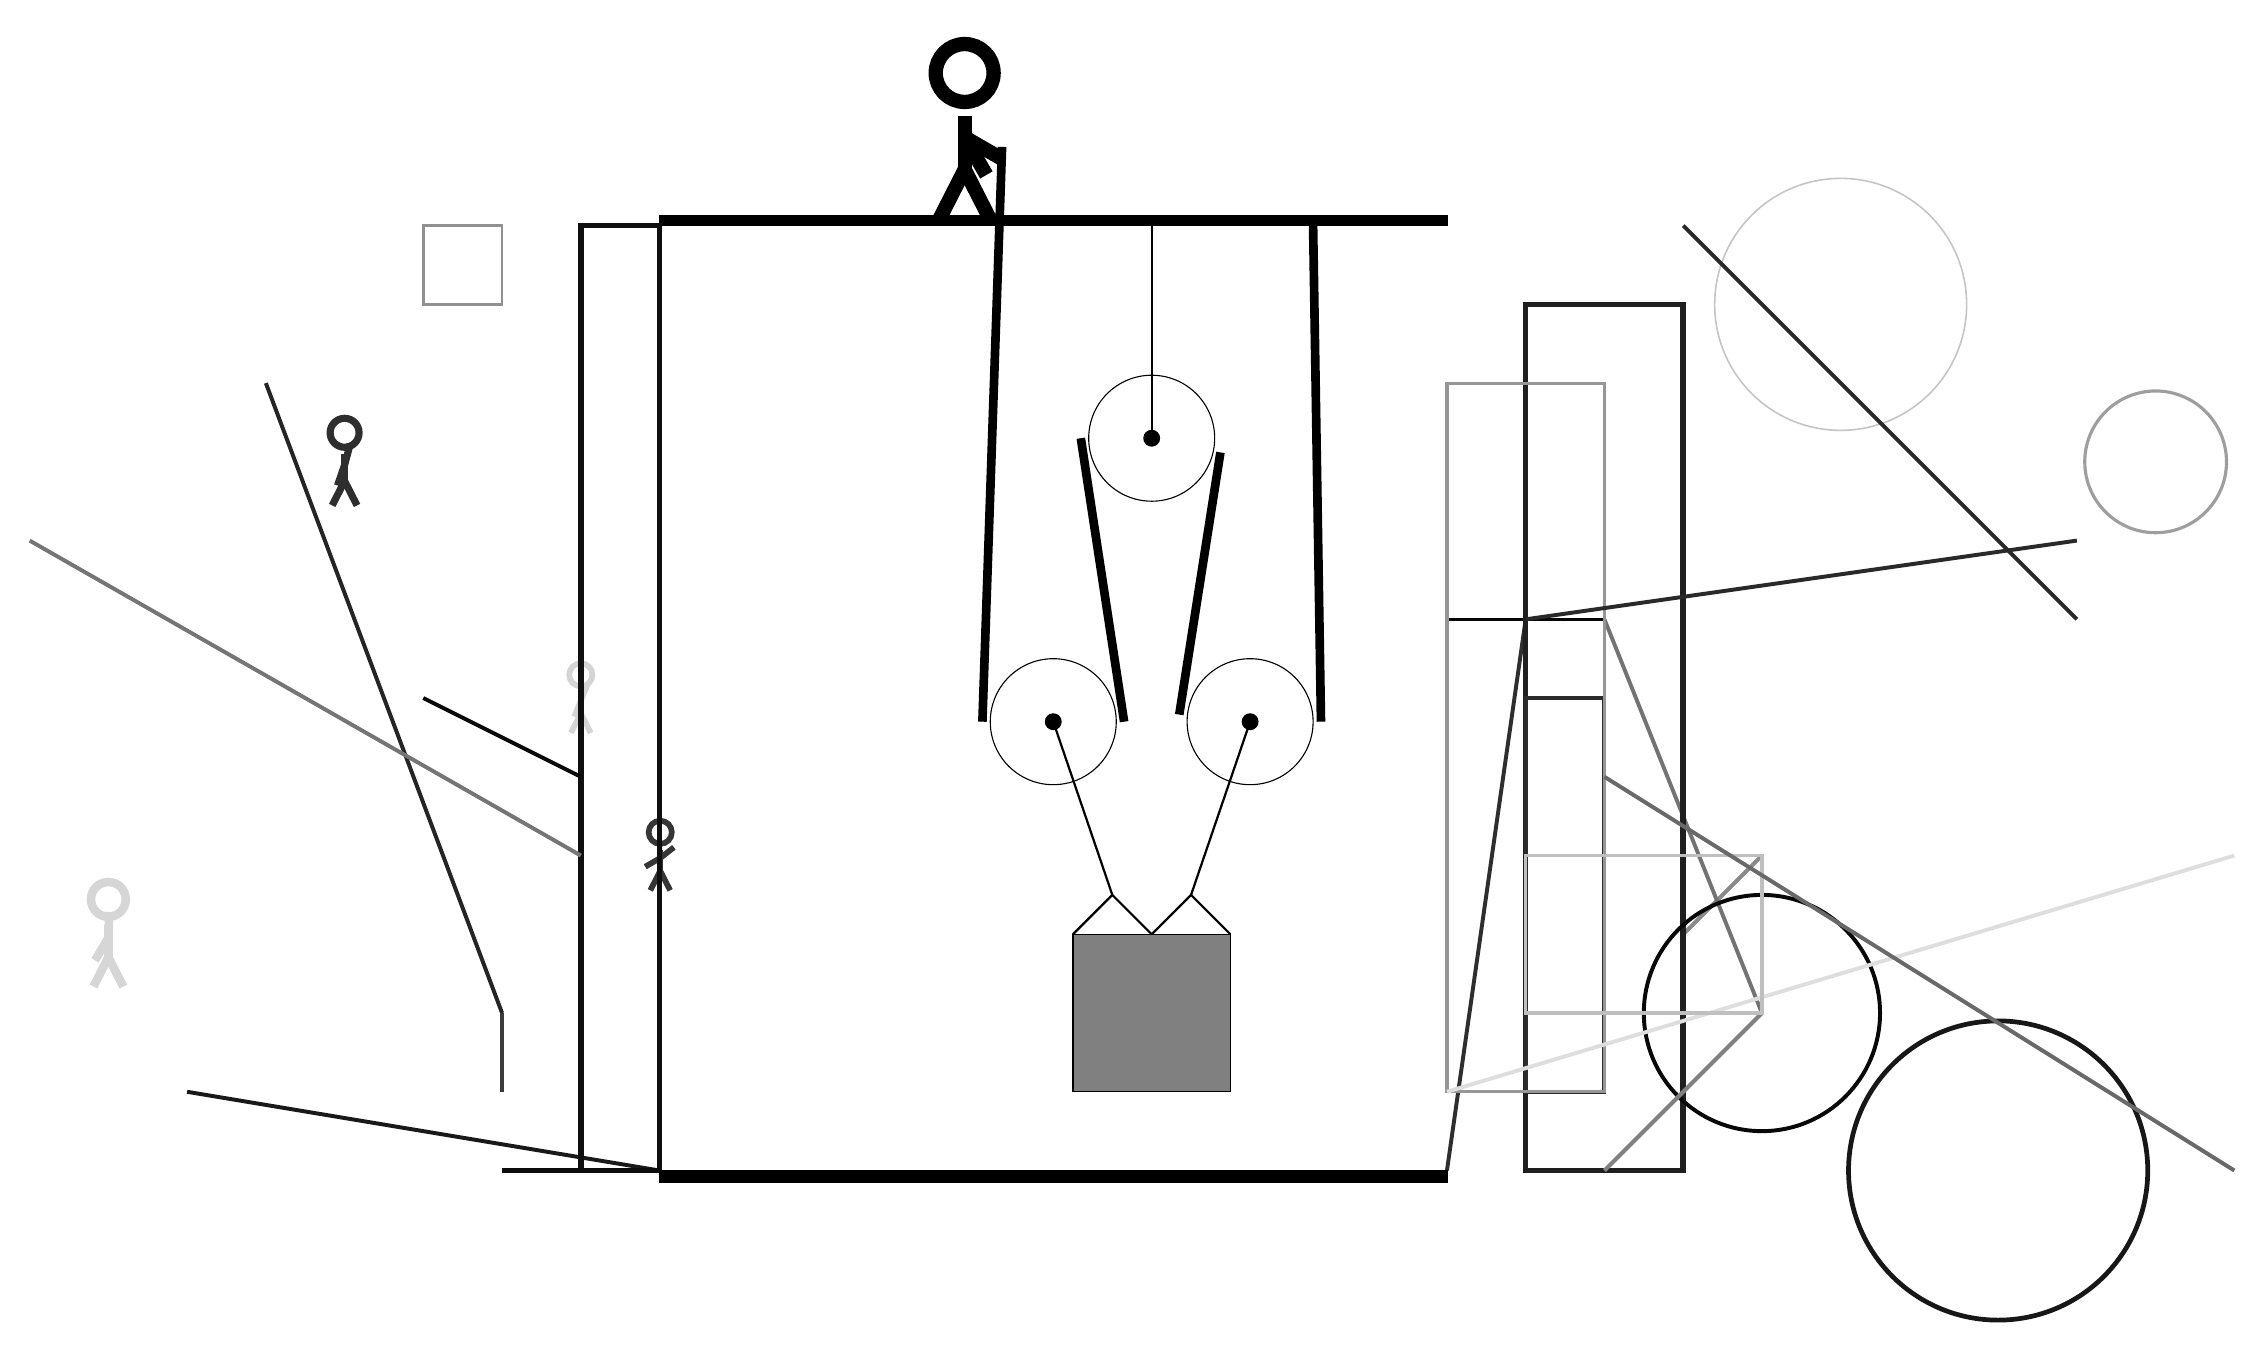
\begin{tikzpicture}
			%%%%% START %%%%%
			
			\draw[fill=black] (-4, 9) rectangle (6, 9.125);
			
			\draw (1, 2.7) circle (0.8);
			\draw[fill=black] (1, 2.7) circle (0.1);
			
			\draw (2.25, 6.3) circle (0.8);
			\draw[fill=black] (2.25, 6.3) circle (0.1);
			\draw[thick] (2.25, 6.3) -- (2.25, 9);
			
			\draw[line width=0.5mm, color=black!46](10, 1) -- (9, 0);
			
			\draw [line width=0.6mm, color=black!91](13, -3) circle (1.9);
			\node[line width=0.7mm, color=black!17] at (-5, 3) {\Strichmaxerl[4][68][67]};
			\draw[line width=0.3mm, color=black!98] (8, 4) rectangle (6, 7);
			\node[line width=0.7mm, color=black!79] at (-4, 1) {\Strichmaxerl[4][30][38]};
			\draw[line width=0.5mm, color=black!86](-6, -1) -- (-9, 7);
			
			\draw[line width=0.5mm, color=black!90](-4, -3) -- (-10, -2);
			\node[line width=0.2mm, color=black!82] at (-8, 6) {\Strichmaxerl[5][71][75]};
			\draw [line width=0.2mm, color=black!23](11, 8) circle (1.6);
			
			\draw[line width=0.7mm, color=black!94] (-5, -3) rectangle (-4, 9);
			
			\draw[line width=0.5mm, color=black!55](10, -1) -- (8, 4);
			\node[line width=0.7mm, color=black!16] at (-11, 0) {\Strichmaxerl[6][59][88]};
			\draw[line width=0.5mm, color=black!82](7, 4) -- (6, -3);
			\draw[line width=0.7mm, color=black!88] (7, 8) rectangle (9, -3);
			\draw[line width=0.5mm, color=black!83] (8, 3) rectangle (7, -2);
			\draw [line width=0.5mm, color=black!97](10, -1) circle (1.5);
			
			\draw[line width=0.3mm, color=black!43] (-6, 9) rectangle (-7, 8);
			\draw[line width=0.4mm, color=black!41] (6, 7) rectangle (8, -2);
			\draw [line width=0.4mm, color=black!38](15, 6) circle (0.9);
			
			\draw[line width=0.5mm, color=black!50](8, -3) -- (10, -1);
			\draw[line width=0.6mm, color=black!77] (-6, -2) rectangle (-6, -1);
			\draw[line width=0.5mm, color=black!54](-5, 1) -- (-12, 5);
			\draw[line width=0.5mm, color=black!84](7, 4) -- (14, 5);
			\draw[line width=0.5mm, color=black!13](6, -2) -- (16, 1);
			\draw[line width=0.4mm, color=black!25] (7, 1) rectangle (10, -1);
			\draw[line width=0.5mm, color=black!59](8, 2) -- (16, -3);
			
			\draw[line width=0.5mm, color=black!84](9, 9) -- (14, 4);
			\draw[line width=0.6mm, color=black!95] (-4, -3) rectangle (-6, -3);
			\draw[line width=0.5mm, color=black!97](-5, 2) -- (-7, 3);
			
			\draw (3.5, 2.7) circle (0.8);
			\draw[fill=black] (3.5, 2.7) circle (0.1);
			
			\draw[thick] (3.5, 2.7) -- (2.75, 0.5);
			\draw[thick] (1, 2.7) -- (1.75, 0.5);
			\draw[thick]  (1.25, 0) -- (1.75, 0.5) -- (2.25, 0);
			\draw[thick]  (2.25, 0) -- (2.75, 0.5) -- (3.25, 0);
			\draw[fill=black!50] (1.25, 0) rectangle (3.25, -2);
			
			\draw[line width=1.1mm] (0.35, 10) --  (0.1, 2.7);
			\centerarc[line width=1.1mm](1, 2.7)(180:360:0.9);
			\draw[line width=1.1mm] (1.9, 2.7) -- (1.35, 6.3);
			\centerarc[line width=1.1mm](2.25, 6.3)(-20:180:0.9);
			\draw[line width=1.1mm](3.123, 6.12) -- (2.6, 2.79);
			\centerarc[line width=1.1mm](3.5, 2.7)(160:360:0.9);
			\draw[line width=1.1mm](4.4, 2.7) -- (4.3, 9);
			
			\node at (-0.07, 10.2) {\Strichmaxerl[10][120][-30]};
			
			\draw[fill=black] (-4, -3) rectangle (6, -3.15);
			
			%%%%% END %%%%%
		\end{tikzpicture}
	\end{figure}	
\end{document}